\appendix
\pagenumbering{Alph}
\renewcommand{\thechapter}{\Alph{chapter}}
\renewcommand{\thesection}{\Roman{section}}
\renewcommand{\thesubsection}{\Roman{subsection}}
\renewcommand\floatpagefraction{0.1}
\clearpage
\chapter{Anhang}
\label{appendix:annex}

\section{Bilder}
\label{annex:images}

\subsection{Einleitung}

\begin{figure}[ht!]
  \begin{centering}
    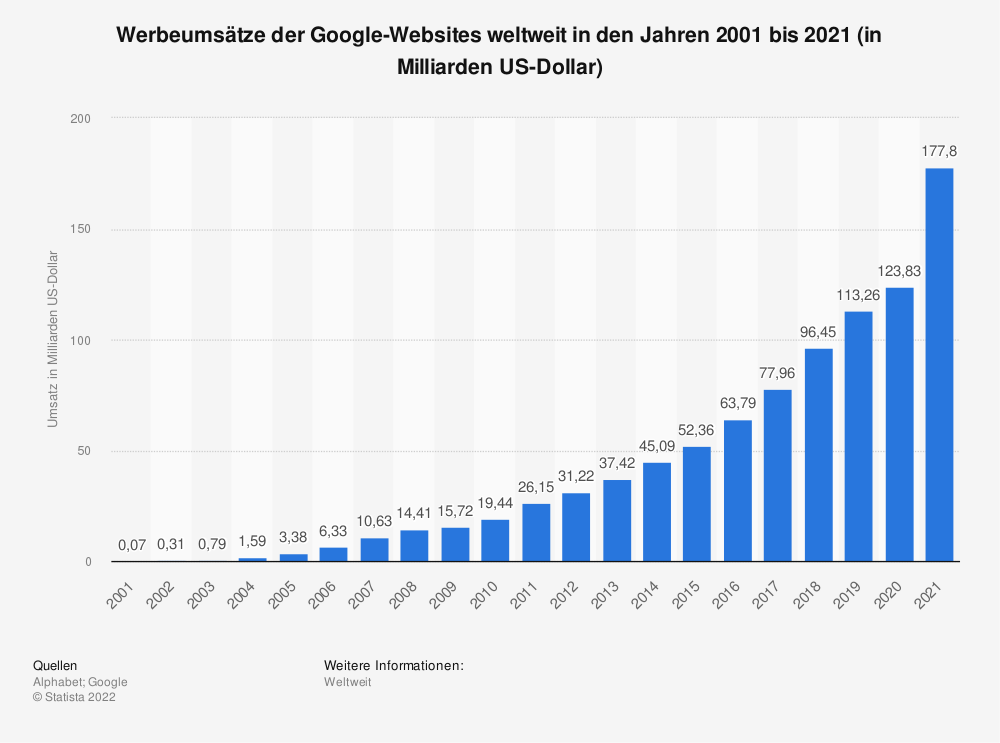
\includegraphics[width=.75\textwidth]{figures/appendix/werbeumsatz.png}
    \caption{Werbeumsätze Google Websites \cite{alphabet2022}}
    \label{fig:werbeumsatz}
  \end{centering}
\end{figure}

\begin{figure}[ht!]
  \begin{centering}
    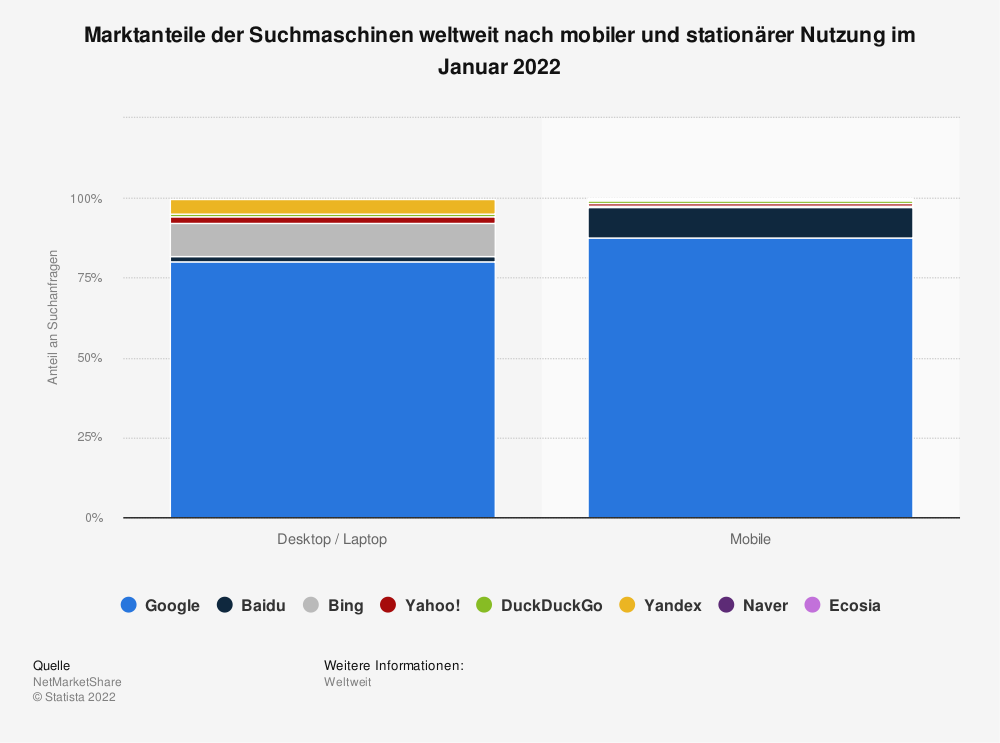
\includegraphics[width=.75\textwidth]{figures/appendix/marketshare.png}
    \caption{Marktanteil Google \cite{netmarketshare2022}}
    \label{fig:marketshare}
  \end{centering}
\end{figure}

\begin{figure}[ht!]
  \begin{centering}
    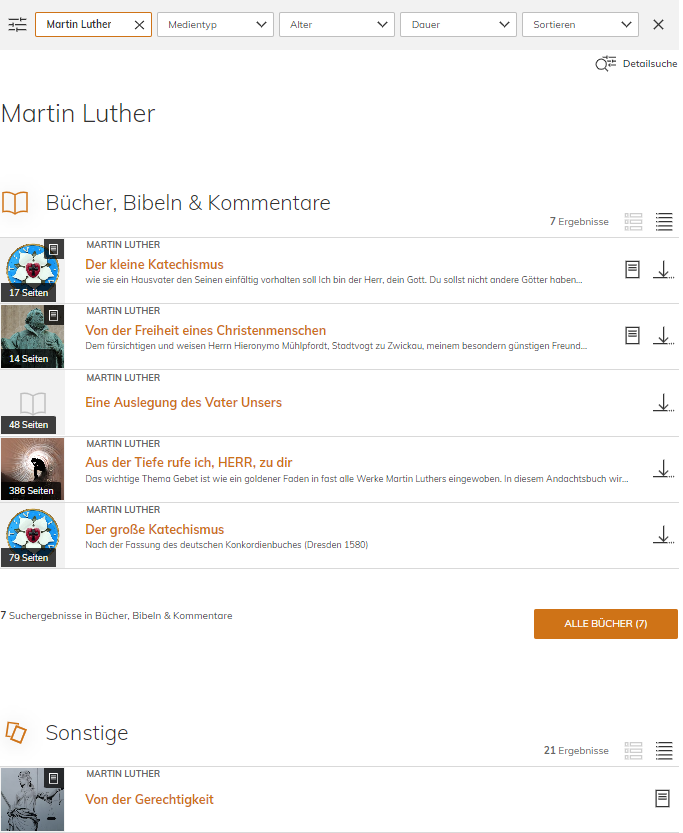
\includegraphics[width=.8\textwidth]{figures/appendix/crossloadSuche.png}
    \caption{Aktuelle Crossload Suche \cite{pfleiderer2022}}
    \label{fig:crossloadSuche}
  \end{centering}
\end{figure}

% 2 Images on one page
% \begin{figure}
%   \includegraphics[width=\textwidth]{figures/appendix/IMAGE.png}
%   \caption{\label{fig:IMAGE} TITLE \cite{CITATION}}
%   \includegraphics[width=\textwidth]{figures/appendix/IMAGE.png}
%   \caption{\label{fig:IMAGE} TITLE \cite{CITATION}}
% \end{figure}

% 1 Images per page
% \begin{figure}
%   \includegraphics[width=\textwidth]{figures/appendix/IMAGE.png}
%   \caption{\label{fig:IMAGE} TITLE \cite{CITATION}}
% \begin{figure}
% \end{figure}
%   \includegraphics[width=\textwidth]{figures/appendix/IMAGE.png}
%   \caption{\label{fig:IMAGE} TITLE \cite{CITATION}}
% \end{figure}


\clearpage
\subsection{Entwicklung}

\begin{figure}[ht!]
  \begin{centering}
    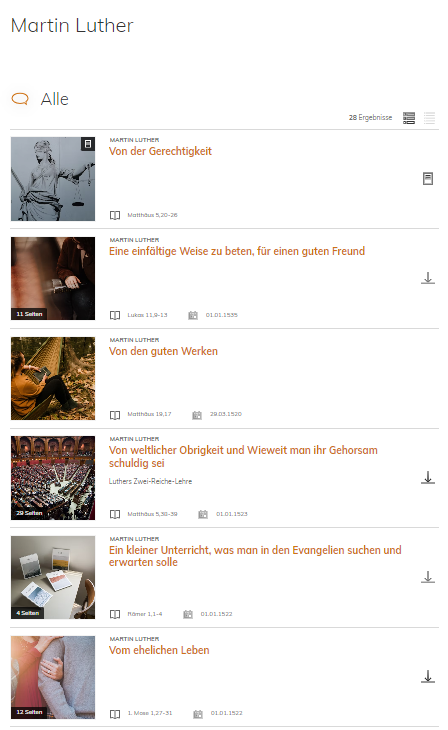
\includegraphics[width=.8\textwidth]{figures/appendix/crossloadSucheNeu.png}
    \caption{Überarbeitete Crossload Suche \cite{pfleiderer2022}}
    \label{fig:crossloadSucheNeu}
  \end{centering}
\end{figure}

\clearpage
\section{Source Code}
\label{annex:sourceCode}

\begin{lstlisting}[language=Java, label=code:SermonCategory, title={Enumeration der verschiedenen Kategorien \cite{frontend2022}}]
  package org.biblepool.search.dto.sermon;

  import java.util.ArrayList;
  import java.util.Arrays;
  import java.util.List;
  import java.util.Objects;
  import java.util.regex.Pattern;
  import java.util.stream.Collectors;

  public enum SermonCategory {
    VIDEO("sermon", Arrays.asList("Video", "Film", "Stream", "Live"), true),
    SERMON("sermon", Arrays.asList("Predigt", "Vortrag", "Mahnwort"), false),
    BOOK("book", Arrays.asList("Buch", "Bücher", "Taschenbuch", "Sammelband", "Reader", "Druck", "Bestseller"), false),
    PICTURE("picture", Arrays.asList("Bild", "Darstellung", "Zeichnung", "Aufnahme", "Foto", "Fotografie"), false),
    MUSIC("music", Arrays.asList("Song", "Melodie", "Hymne", "Stück", "Gesang", "Klavier", "Musik", "Orchester"), false),
    AUDIOBOOK("audio", Arrays.asList("Hörbuch", "Hörbücher", "Audiobook"), false),
    OTHER("other", Arrays.asList("Sonstige", "Andere"), false);

    private String id;
    private Boolean hasVideo;
    private List<String> synonyms = new ArrayList<>();
    private Pattern pattern;

    public static List<SermonCategory> getAllCategories() {
      return Arrays.asList(SermonCategory.values());
    }

    private SermonCategory(String id, List<String> synonyms, Boolean hasVideo) {
      setId(id);
      setSynonyms(synonyms);
      setHasVideo(hasVideo);
    }

    public List<String> getSynonyms() {
      return synonyms;
    }

    public void setSynonyms(List<String> synonyms) {
      if(Objects.isNull(getSynonyms())) {
        this.synonyms = new ArrayList<>();
      }
      else {
        this.synonyms = synonyms;
      }
    }

    public String getId() {
      return id;
    }

    public void setId(String id) {
      this.id = id;
    }

    public Boolean hasVideo() {
      return hasVideo;
    }

    public void setHasVideo(Boolean hasVideo) {
      this.hasVideo = hasVideo;
    }

    public void setPattern() {
      String regex = synonyms.stream().collect(Collectors.joining("|"));
      pattern = Pattern.compile("(" + regex + ")", Pattern.CASE_INSENSITIVE);
    }

    public boolean hasCategory(String term) {
      return pattern.matcher(term).matches();
    }
  }

\end{lstlisting}

\clearpage

\begin{lstlisting}[language=Java, label=code:SolrResponse, title={Vorschlag in der zurückgegebenen Antwort \cite{solr-search2022}}]
  package org.biblepool.search.business.paging;

  import org.biblepool.schema.api.sermon.dto.Sermon;

  import java.util.List;
  public class Page {

    private Meta meta;
    private List<Sermon> content;
    private Sermon suggestion;

    public Sermon parseSuggestion(List<Sermon> mostRelevant) {
      // Case 0: If there is only one content in the list, return that as suggestion
      boolean onlyOneElement = mostRelevant.size() == 1;

      // Case 1: Score of the first element is at least twice as much of the second score
      boolean biggerThanDoubleTheScore = mostRelevant.size() > 2 && mostRelevant.get(0).getScore() >= 2 * mostRelevant.get(1).getScore();

      if(onlyOneElement || biggerThanDoubleTheScore) {
        return mostRelevant.get(0);
      }

      // Case 2: Get the average of the most relevant sermons and check if the first has at least twice as much of that
      if(!mostRelevant.isEmpty()) {
        Float average = (float) mostRelevant
          .stream()
          .mapToDouble(sermon -> sermon.getScore())
          .summaryStatistics()
          .getAverage();

        if(mostRelevant.get(0).getScore() >= 2 * average) {
          return mostRelevant.get(0);
        }
      }

      return null;
    }

    public Meta getMeta() {
      return meta;
    }

    public void setMeta(Meta meta) {
      this.meta = meta;
    }

    public List<Sermon> getContent() {
      return content;
    }

    public void setContent(List<Sermon> content) {
      this.content = content;
    }

    public Sermon getSuggestion() {
      return suggestion;
    }

    public void setSuggestion(Sermon suggestion) {
      this.suggestion = suggestion;
    }
  }
\end{lstlisting}

% \begin{lstlisting}[language=Java, label=code:, title={ \cite{}}]

% \end{lstlisting}
